\documentclass{article}

\usepackage[spanish]{babel}
\usepackage[numbers,sort&compress]{natbib}
\usepackage[T1]{fontenc}
\usepackage[ansinew]{inputenc}
\usepackage{graphicx}
\usepackage{url}

\title { Movimiento Browniano}
\author{Oscar Quinonez}

\begin{document}

\maketitle

\section{Introducci\'on}\label{intro}

El movimiento browniano es el comportamiento caotico y erratico  llevado a cabo por una part\'icula muy chica que esta inmersa en un fluido, se llama as\'i en honor al franc\'es Robert Brown, bi\'ologo y bot\'anico. Su principal caracteriztica es la trayectoria irregular en foma de zigzag. El f\'isico franc\'es Jean Perrin (1870-1942) dio una bella descripci\'on de este fen\'omeno: "En un fluido en equilibrio, como el agua dentro de un vaso, todas sus partes aparecen completamente sin movimiento. Si ponemos en el agua un objeto de mayor densidad, cae. La ca\'ida, es cierto, ser\'a m\'as lenta si el objeto es menor; pero un objeto visible siempre termina en el fondo del vaso y no tiende a subir. Sin embargo, ser\'ia dif\'icil examinar durante mucho tiempo una preparaci\'on de part\'iculas muy finas en un l\'iquido sin observar un movimiento perfectamente irregular. Se mueven, se detienen, empiezan de nuevo, suben, bajan, suben otra vez, sin que se vea que tiendan a la inmovilidad".\cite{baz}.
El estudio del movimiento browniano ha ejercido una poderosa influencia en fisica, quimica y matematicas, por ejemplo, Albert Einstein lo us\'o como m\'etodo de observaci\'on concluyente para la confirmaci\'on de la teoria at\'omica de la materia, adem\'as que la medici\'on de ciertas propiedades del movimiento browniano determinaba diversas constantes f\'isicas de importancia: las masas de los \'atomos y las moleculas y el valor del n\'umero de Avogadro. \citet{mov}.
Actualmente el movimiento browniano se encuentra muy presente en suspensiones coloidales y ha sido adaptado para modelos matematicos en finanzas para calcular riesgos en el mercado.\citep{dat}.
 
\section{Objetivo}\label{met}

A traves de esta simulaci\'on se intent\'o representar la manera en que afecta la dimensi\'on en el regreso de una part\'icula a su origen, se simularon hasta 8 dimensiones dentro de los que se cambi\'o la cantidad de pasos con potencias de 2, estas potencias se encontraban entre 5 a 10 veces en incremento de uno, en total se llevaron a cabo 50 repeticiones de la simulaci\'on para cada incremento.

\section{Metodolog\'ia}\label{met}

Para llevar a cabo la simulaci\'on del movimiento browniano se utiliz\'o el programa R 4.0.2 para representar una caminata desde el origen, es decir, cada paso de la caminata representaba un tiempo, fueron simuladas hasta 8 dimensiones con los incrementos exponenciales antes mencionados entre 5 y 10, a cada incremento se le hicieron 50 repeticiones para conocer que tan probable podr\'ia ser el retorno al origen de la part\'icula.
En las gr\'aficas adjuntas se puede observar como afectaron las 8 dimensiones en el tiempo que le tom\'o a la part\'icula regresar a su origen.
 
\section{Resultados y Discusi\'on}\label{res}

Al realizar la simulaci\'on en R 4.0.2 se gener\'o una serie de datos que explican el porcentaje de regreso de la part\'icula al origen en cada una de las 8 dimensiones y la duracion de la serie de pasos conocida como caminata, estos datos se muestran en la tabla 1.
Los datos fueron represntados de mejor manera en las graficas de caja-bigote. En la figura 1 \ref{f1} se representan las 8 dimensiones y como la particula se comporta dentro de cada una, siendo cada caja la representaci\'on de una dimensi\'on distinta. Mientras en la figura 2 \ref{f2} se puede observar la distancia que alcanz\'o a recorrer la part\'icula en cada una de las 8 dimensiones dentro de las que fue simulada.
 
\begin{table}
 \caption{Datos generadoss en R.}
 \label{t1}
 \begin{center}
 \begin{tabular}{rrr}
\texttt{pot} & \texttt{porc} & \texttt{dim} \\

5  &  100  &  1  \\
5  &  66  &  2  \\
5  &  40  &  3  \\
5  &  22  &  4  \\
5  &  14  &  5  \\
5  &  8  &  6  \\
5  &  6  &  7  \\
5  &  6  &  8  \\
6  &  98  &  1  \\
6  &  74  &  2  \\
$\vdots$ &   $\vdots$ &   $\vdots$ \\    
10  &  96  &  1  \\
10  &  68  &  2  \\
10  &  32  &  3  \\
10  &  20  &  4  \\
10  &  4  &  5  \\
10  &  6  &  6  \\
10  &  6  &  7  \\
10  &  4  &  8  \\
\end{tabular}
\end{center}
\end{table}

\begin{figure}

 \begin{center}
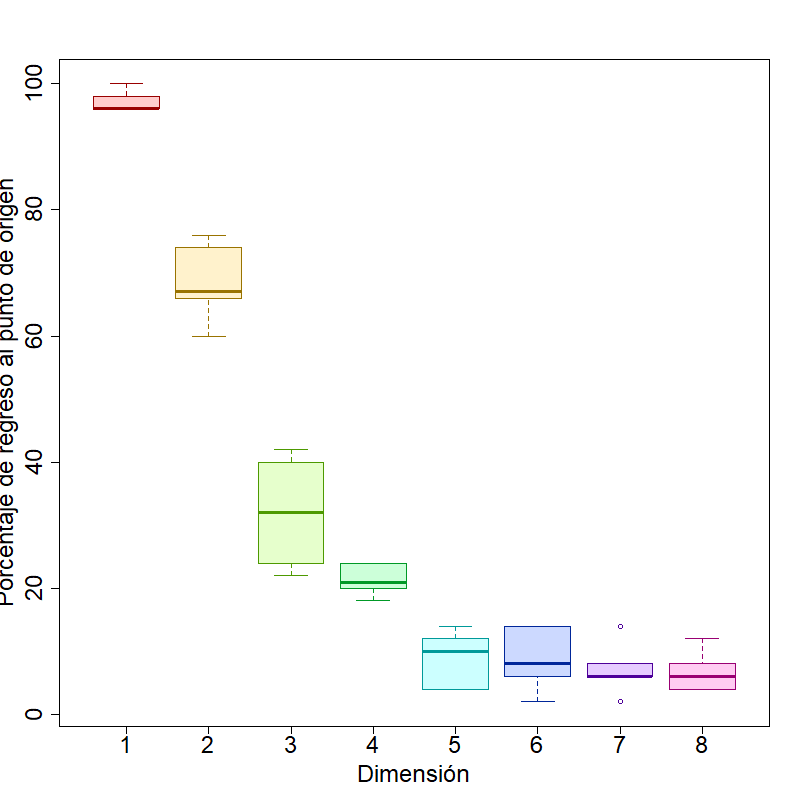
\includegraphics[scale=0.3]{tareaunosim.png}
\end{center}
  \caption{Probabilidad de regreso por dimensi\'on.}
  \label{f1}
  
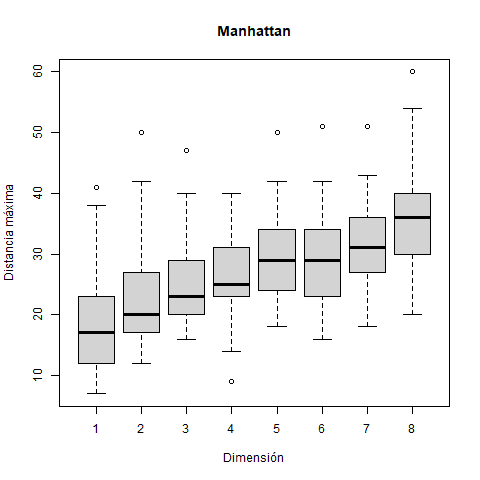
\includegraphics[scale=0.5]{tareaunomr.png}
 \caption{Distancia maxima.}
  \label{f2}
 
\end{figure}
 
\newpage

\section{Conclusiones}

La simulaci\'on de modelos matematicos usando R 4.0.2 nos ayuda a observar de cierta manera el comportamiento de una part\'icula a la que le afectan 8 dimensiones y la cantidad de pasos dentro de la caminata, dentro de este comportamiento analizamos la distancia maxima de recorrido asi como el porcentaje de retorno de la part\'icula al origen y por simple deducci\'on, mientras mas dimensiones sean simuladas  mas complicada ser\'a que vuelva a dicho origen.

\bibliography{intento1}
\bibliographystyle{plainnat}


\end{document}